\documentclass[11pt]{article}
\usepackage{graphicx}
\usepackage[utf8]{inputenc}
\usepackage{amsmath}
\usepackage{amssymb}
\usepackage{gensymb}
\usepackage{geometry}
\graphicspath{ {../img/} }
\numberwithin{equation}{section}
\geometry{
	total={210mm,297mm},
	left=35mm,
	right=35mm,
	top=35mm,
	bottom=35mm,
}
\def\note_1{\footnote{Voici l'équation utilisée pour dessiner le graphique :\\\center$z(x,y) = \mathrm{cos}(\frac{2\pi}{\lambda}\sqrt{(x-2)^2+y^2})+\mathrm{cos}(\frac{2\pi}{\lambda}\sqrt{(x+2)^2+y^2})$}}

\begin{document}
Voici le schéma\note_1 du problème si l'on peut visualiser les ondes sonores provenant des deux sources de même fréquences :
\begin{figure}[h]
	\caption{Interférence visualisée}
	\centering
	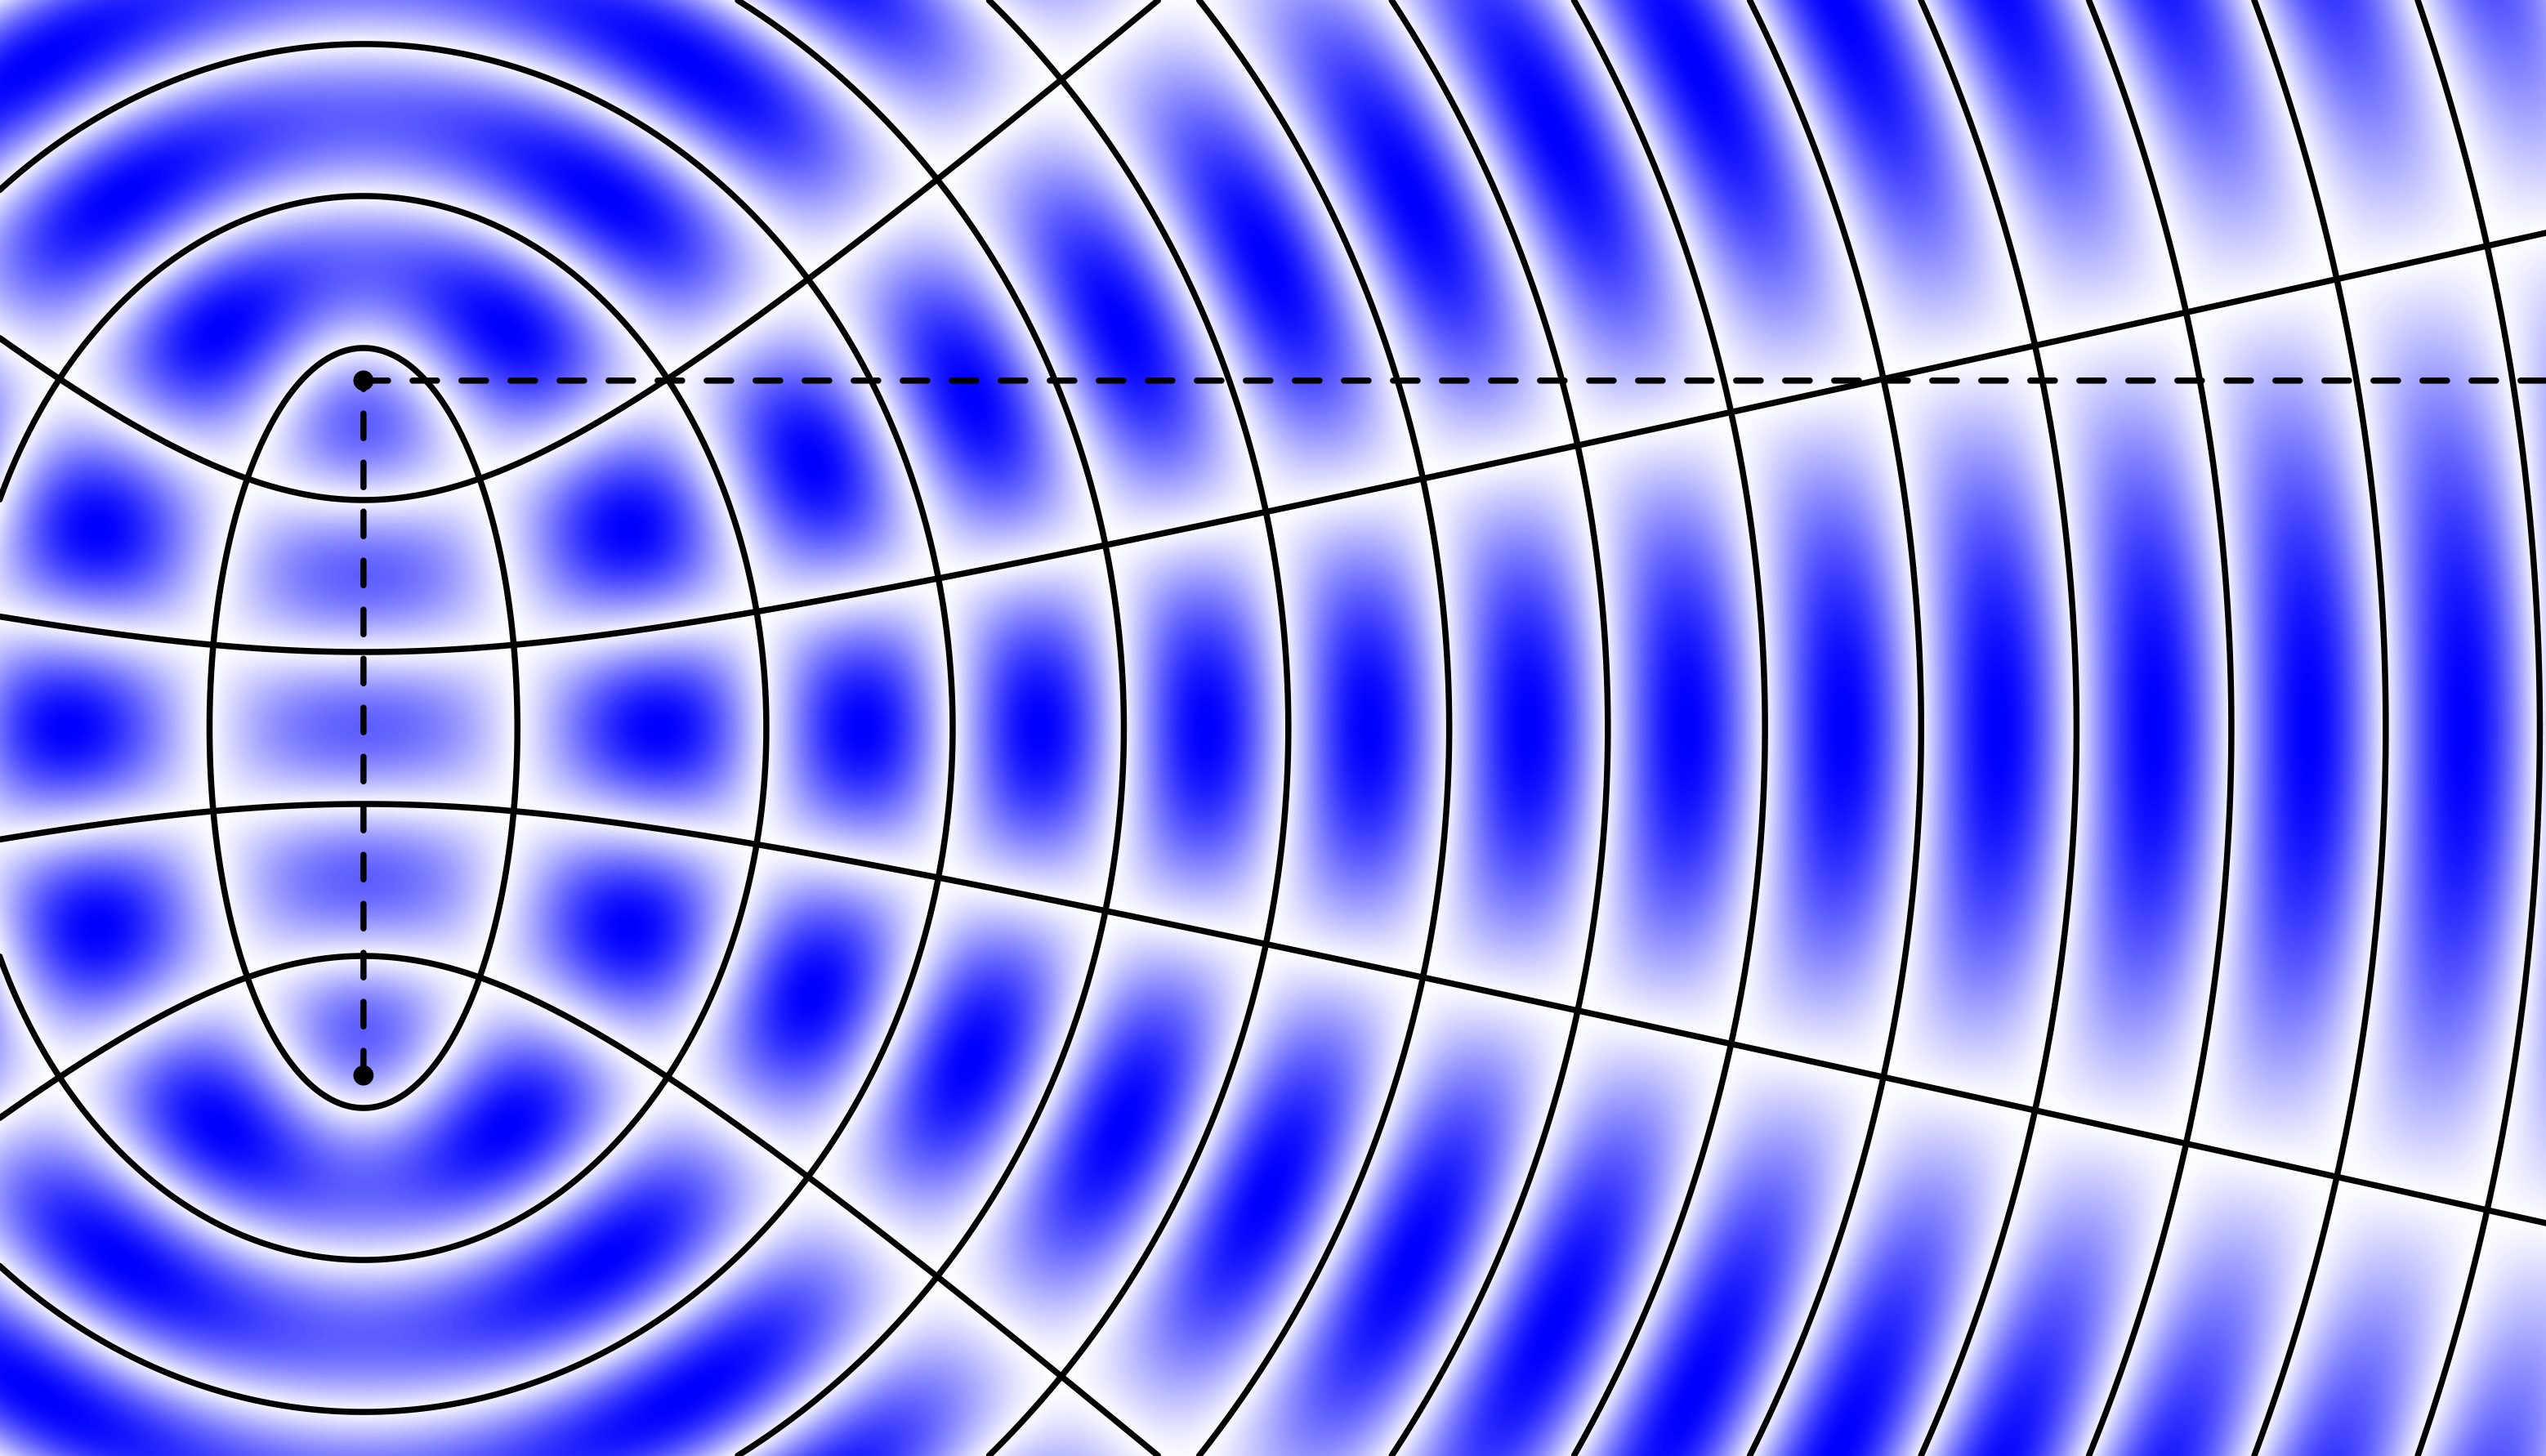
\includegraphics[scale=0.1]{plot.png}
\end{figure}

À partir de cette image, on peut clairement voir qu'il existe seulement deux minimums sonores dans le trajet de la personne. Il faut donc le prouver. Pour ce faire, il nous suffit de trouver le nombre de valeur de $x$ pour lesquelles il est possible d'avoir une différence de marche équivalente à une demi longueur d'onde.\\

Avec pythagore, on peut déterminer la différence de marche entre le haut-parleur en diagonal et celui en face de la personne :
\begin{equation*}
	\Delta r=\sqrt{x^2+d^2}-x\\
\end{equation*}

Afin d'avoir un minimum, la différence de marche doit être équivalente à un multiple d'une demi longueur d'onde :
\begin{equation*}
	\Delta r=\sqrt{x^2+d^2}-x=\left (n+\frac{1}{2}\right )\lambda\\
\end{equation*}
\pagebreak

Il suffit de résoudre l'équation :
\begin{alignat*}{3}
	                     & & \sqrt{x^2+d^2}-x&=\left (n+\frac{1}{2}\right )\lambda\\
	\Leftrightarrow\quad & & \sqrt{x^2+d^2}  &=\left (n+\frac{1}{2}\right )\lambda+x\\
	\Rightarrow\quad     & &       x^2+d^2   &=\left [\left (n+\frac{1}{2}\right )\lambda+x\right ]^2\\
    \Leftrightarrow\quad & &       x^2+d^2   &=\left [\left (n+\frac{1}{2}\right )\lambda\right ]^2+2x\left (n+\frac{1}{2}\right )\lambda+x^2\\
    \Leftrightarrow\quad & &       d^2       &=\left [\left (n+\frac{1}{2}\right )\lambda\right ]^2+2x\left (n+\frac{1}{2}\right )\lambda\\
    \Leftrightarrow\quad & & 2x\left (n+\frac{1}{2}\right )\lambda&=d^2-\left [\left (n+\frac{1}{2}\right )\lambda\right ]^2\\
    \Leftrightarrow\quad & & x &=\frac{d^2-\left [\left (n+\dfrac{1}{2}\right )\lambda\right ]^2}{2\left (n+\dfrac{1}{2}\right )\lambda}\quad\quad\text{si $n=0,1,2,...$}\\
\end{alignat*}

On s'intéresse aux valeurs de $x$ lorsque la personne est devant les deux haut-parleurs. En analysant la fonction, on remarque qu'elle est positive si et seulement si l'expression au carré est plus petite que $d^2$, la distance entre les deux sources. En termes mathématiques :
\begin{equation*}
	\left [\left (n+\dfrac{1}{2}\right )\lambda\right ]^2<d^2\\
\end{equation*}

Le seul inconnue est $n$, on peut donc l'isoler afin d'obtenir pour quelles valeurs de $n$ des valeurs de $x$ existent.
\begin{alignat*}{3}
	                     & & \left [\left (n+\dfrac{1}{2}\right )\lambda\right ]^2&<d^2\\
	\Rightarrow\quad     & &        \left (n+\dfrac{1}{2}\right )\lambda          &<d\\
	\Leftrightarrow\quad & &               n                                      &<\frac{d}{\lambda}-\frac{1}{2}\quad\quad\text{si $\lambda=\frac{v}{f}$}\\
	\Leftrightarrow\quad & &               n                                      &<\frac{d\cdot f}{v}-\frac{1}{2}=\frac{4\mathrm{m}\cdot 200\mathrm{Hz}}{343\mathrm{m/s}}-\frac{1}{2}=1.83\\
\end{alignat*}

Puisque $n$ doit être un nombre entier positif, seulement $n=0$ et $n=1$ respectent les conditions du problèmes. Il y a donc seulement deux minimums possibles et non trois.
\end{document}
